\documentclass[12pt]{article}


\usepackage{amssymb}
\usepackage{amsmath}
\usepackage{fullpage}
\usepackage{epsfig}
\usepackage{epstopdf, xcolor, hyperref}
\everymath{\displaystyle}
\usepackage{enumerate}



\begin{document}

\begin{center}
\underline{\LARGE{Partial Derivatives}}
\end{center}

\noindent SUGGESTED REFERENCE MATERIAL:

\bigskip

\noindent As you work through the problems listed below, you should reference Chapter 13.3 of the recommended textbook (or the equivalent chapter in your alternative textbook/online resource) and your lecture notes.

\bigskip

\noindent EXPECTED SKILLS:

\begin{itemize}

\item Be able to compute first-order and second-order partial derivatives. 

\item Be able to perform implicit partial differentiation. 

\item Be able to solve various word problems involving rates of change, which use partial derivatives.

\end{itemize}

\noindent PRACTICE PROBLEMS:

\medskip

\begin{enumerate}

\item A portion of the surface defined by $z=f(x,y)$ is shown below.

\begin{center}
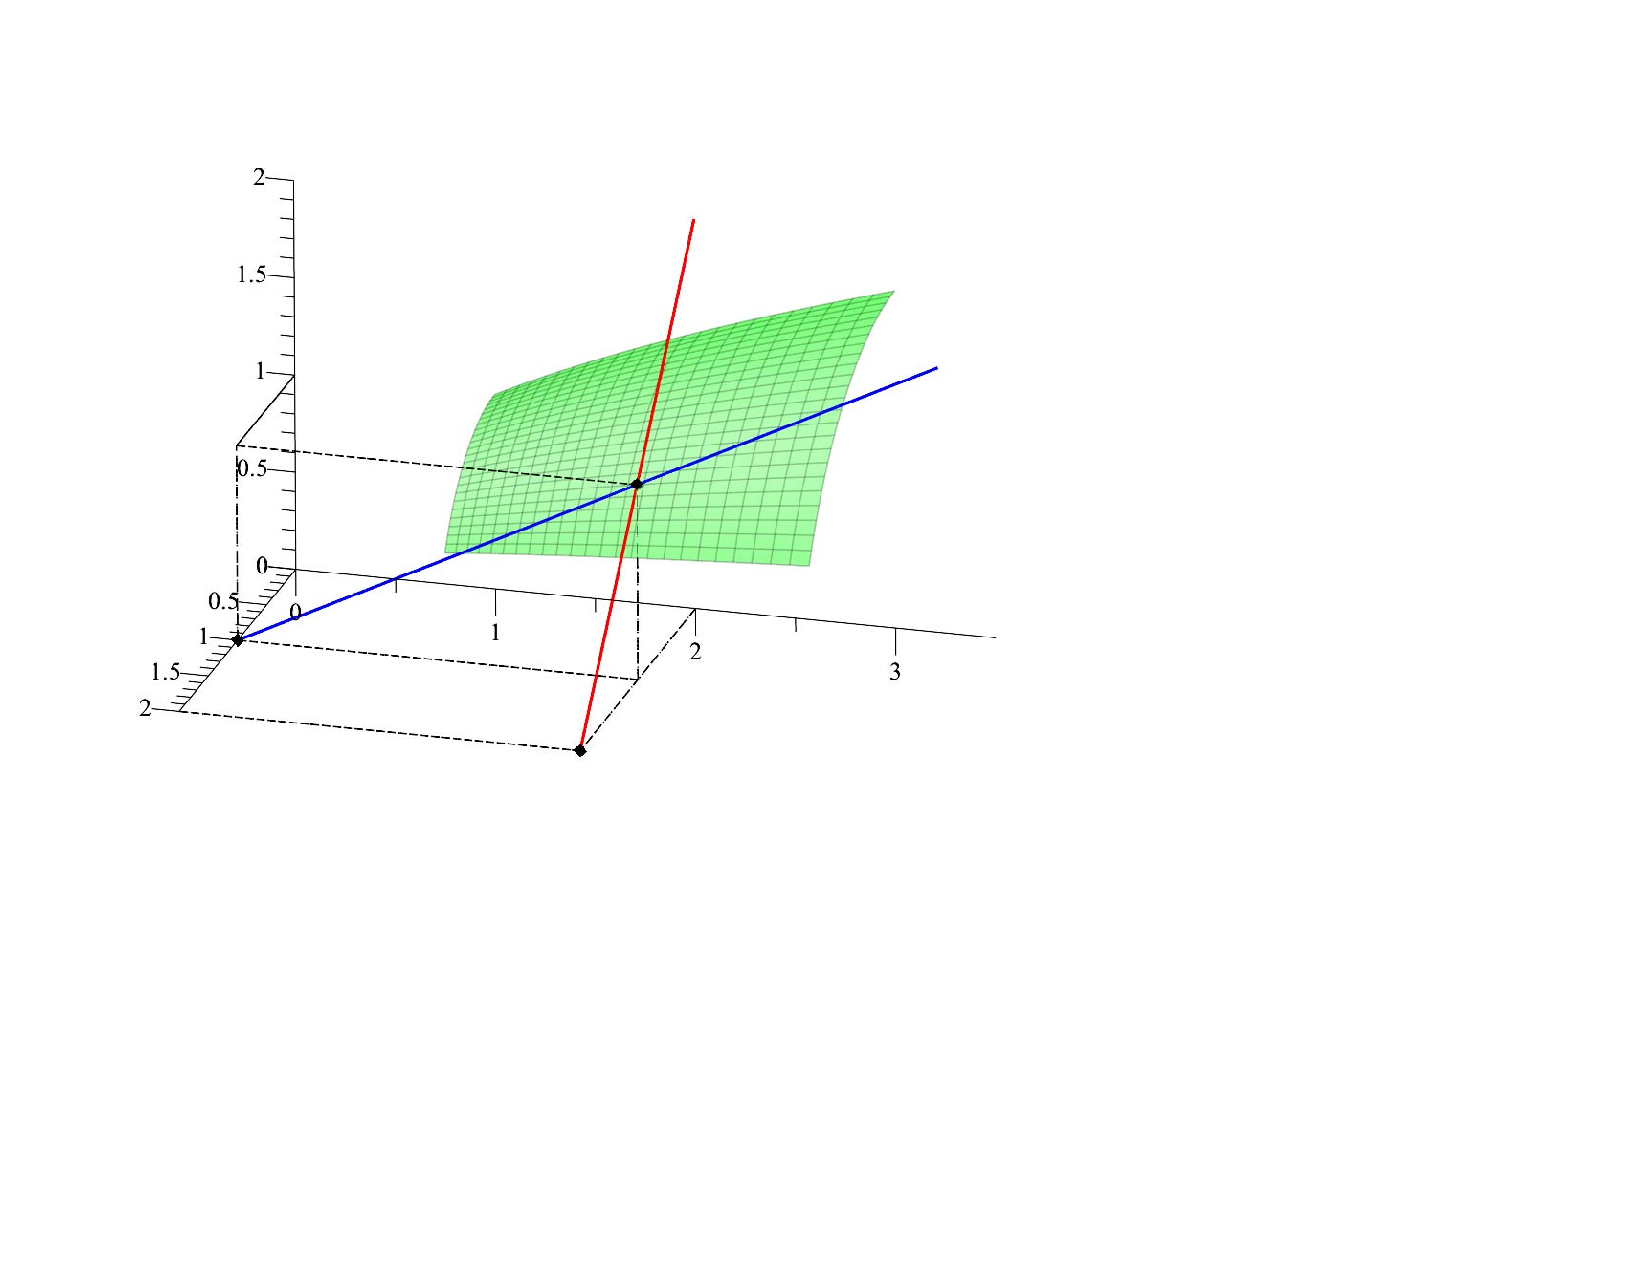
\includegraphics[scale=0.6]{tangents2.pdf}
\end{center}

Use the tangent lines in this figure to calculate the values of the first order partial derivatives of $f$ at the point $(1,2)$.

\includegraphics[scale=0.5]{start.pdf}
{{$f_x(1,2)=-1$; $f_y(1,2)=\frac{1}{2}$}}
\includegraphics[scale=0.5]{end.pdf}


\end{enumerate}

\newpage

\noindent {\bf For problems 2-9, find all first order partial derivatives.}

\begin{enumerate}
\setcounter{enumi}{1}

\item $f(x,y)=(3x-y)^5$

\includegraphics[scale=0.5]{start.pdf}
{{$f_x(x,y)=15(3x-y)^4$; $f_y(x,y)=-5(3x-y)^4$}}
\includegraphics[scale=0.5]{end.pdf}


\item $f(x,y)=e^x\sin{y}$

\includegraphics[scale=0.5]{start.pdf}
{{$f_x(x,y)=e^x\sin{y}$; $f_y(x,y)=e^x\cos{y}$}}
\includegraphics[scale=0.5]{end.pdf}


\item $f(x,y)=\tan^{-1}{(4x-7y)}$

\includegraphics[scale=0.5]{start.pdf}
{{$f_x(x,y)=\frac{4}{1+(4x-7y)^2}$; $f_y(x,y)=-\frac{7}{1+(4x-7y)^2}$}}
\includegraphics[scale=0.5]{end.pdf}


\item $f(x,y)=x\cos{(x^2+y^2)}$

\includegraphics[scale=0.5]{start.pdf}
{{$f_x(x,y)=\cos{(x^2+y^2)}-2x^2\sin{(x^2+y^2)}$; $f_y(x,y)=-2xy\sin{(x^2+y^2)}$}}
\includegraphics[scale=0.5]{end.pdf}


\item Let $f(x,y,z)=\sqrt{x^2-2y+3z^2}$.  Compute $\frac{\partial f}{\partial x}$,  $\frac{\partial f}{\partial y}$, and $\frac{\partial f}{\partial z}$.

\includegraphics[scale=0.5]{start.pdf}
{{$\frac{\partial f}{\partial x}=\frac{x}{\sqrt{x^2-2y+3z^2}}$; $\frac{\partial f}{\partial y}=\frac{-1}{\sqrt{x^2-2y+3z^2}}$; $\frac{\partial f}{\partial z}=\frac{3z}{\sqrt{x^2-2y+3z^2}}$}}
\includegraphics[scale=0.5]{end.pdf}


\item Let $w=\frac{4z}{x^2+y^2}$.  Compute $\frac{\partial w}{\partial x}$, $\frac{\partial w}{\partial y}$, and $\frac{\partial w}{\partial z}$.

\includegraphics[scale=0.5]{start.pdf}
{{$\frac{\partial w}{\partial x}=-\frac{8xz}{(x^2+y^2)^2}$; $\frac{\partial w}{\partial y}=-\frac{8yz}{(x^2+y^2)^2}$; $\frac{\partial w}{\partial z}=\frac{4}{x^2+y^2}$}}
\includegraphics[scale=0.5]{end.pdf}


\item Consider $f(x,y,z)=\frac{xy}{x^2+z^2}$.  Determine $\frac{\partial f}{\partial x}(-1, 1, 2)$, $\frac{\partial f}{\partial y}(-1, 1, 2)$, and $\frac{\partial f}{\partial z}(-1, 1, 2)$.

\includegraphics[scale=0.5]{start.pdf}
{{$\left.\frac{\partial f}{\partial x}\right|_{(x,y,z)=(-1,1,2)}=\frac{3}{25}$; $\left.\frac{\partial f}{\partial y}\right|_{(x,y,z)=(-1,1,2)}=-\frac{1}{5}$; $\left.\frac{\partial f}{\partial z}\right|_{(x,y,z)=(-1,1,2)}=\frac{4}{25}$}}
\includegraphics[scale=0.5]{end.pdf}


\item Suppose $f(x,y,z)=z^2\sin{(2xy)}$.  Compute $f_x\left(4, \frac{\pi}{3}, 1\right)$, $f_y\left(4, \frac{\pi}{3}, 1\right)$, and $f_z\left(4, \frac{\pi}{3}, 1\right)$.

\includegraphics[scale=0.5]{start.pdf}
{{$f_x\left(4,\frac{\pi}{3},1\right)=-\frac{\pi}{3}$, $f_y\left(4,\frac{\pi}{3},2\right)=-4$, $f_z\left(4,\frac{\pi}{3},2\right)=\sqrt{3}$} }
\includegraphics[scale=0.5]{end.pdf}


\end{enumerate}

\noindent {\bf For problems 10-11, find all values of $x$ and $y$ such that $f_x(x,y)=0$ and $f_y(x,y)=0$ simultaneously. }

\begin{enumerate}
\setcounter{enumi}{9}

\item $f(x,y)=4x^2+y^2-8xy+4x+6y-10$ 

\includegraphics[scale=0.5]{start.pdf}
{{$(x,y)=\left(\frac{7}{6},\frac{5}{3}\right)$}}
\includegraphics[scale=0.5]{end.pdf}


\item $f(x,y)=x^2+4y^2-3xy+3$ 

\includegraphics[scale=0.5]{start.pdf}
{{$(x,y)=(0,0)$}}
\includegraphics[scale=0.5]{end.pdf}


\end{enumerate}

\noindent {\bf For problems 12-13, compute all second partial derivatives.}

\begin{enumerate}
\setcounter{enumi}{11}

\item $z=x^2y-y^3x^4$ 

\includegraphics[scale=0.5]{start.pdf}
{{$\frac{\partial^2z}{\partial x^2}=2y-12x^2y^3$; $\frac{\partial^2z}{\partial y \partial x}=2x-12x^3y^2$; $\frac{\partial^2z}{\partial x \partial y}=2x-12x^3y^2$; $\frac{\partial^2z}{\partial y^2}=-6x^4y$}}
\includegraphics[scale=0.5]{end.pdf}


\item $f(x,y)=\ln{(x^2+3y)}$ 

\includegraphics[scale=0.5]{start.pdf}
{{{0.6\linewidth}{$f_{xx}(x,y)=\frac{-2x^2+6y}{(x^2+3y)^2}$; $f_{xy}(x,y)=-\frac{6x}{(x^2+3y)^2}$;\\ $f_{yx}(x,y)=-\frac{6x}{(x^2+3y)^2}$; $f_{yy}(x,y)=-\frac{9}{(x^2+3y)^2}$}}}
\includegraphics[scale=0.5]{end.pdf}


\item Consider the surface $S: z=x^2+3y^2$.  

\begin{enumerate}

\item Find the slope of the tangent line to the curve of intersection of the surface $S$ and the plane $y=1$ at the point $(1,1,4)$.

\includegraphics[scale=0.5]{start.pdf}
{{2; Detailed Solution: \textcolor{blue}{\href{http://www.math.drexel.edu/classes/Calculus/resources/Math200HW/Solutions/10_200_Partial_14.pdf}{Here}} }}
\includegraphics[scale=0.5]{end.pdf}


\item Find a set of parametric equations for the tangent line whose slope you computed in part (a).  

\includegraphics[scale=0.5]{start.pdf}
{{{1\linewidth}{There are many possible parameterizations.  One possibility is $x=1+t$, $y=1$, $z=4+2t$. Detailed Solution: \textcolor{blue}{\href{http://www.math.drexel.edu/classes/Calculus/resources/Math200HW/Solutions/10_200_Partial_14.pdf}{Here}} }}}
\includegraphics[scale=0.5]{end.pdf}


\item Find the slope of the tangent line to the curve of intersection of the surface $S$ and the plane $x=1$ at the point $(1,1,4)$.

\includegraphics[scale=0.5]{start.pdf}
{{6; Detailed Solution: \textcolor{blue}{\href{http://www.math.drexel.edu/classes/Calculus/resources/Math200HW/Solutions/10_200_Partial_14.pdf}{Here}} }}
\includegraphics[scale=0.5]{end.pdf}


\item Find a set of parametric equations for the tangent line whose slope you computed in part (b).  

\includegraphics[scale=0.5]{start.pdf}
{{{1\linewidth}{There are many possible parameterizations.  One possibility is $x=1$, $y=1+t$, $z=4+6t$. Detailed Solution: \textcolor{blue}{\href{http://www.math.drexel.edu/classes/Calculus/resources/Math200HW/Solutions/10_200_Partial_14.pdf}{Here}} }}}
\includegraphics[scale=0.5]{end.pdf}


\item Find an equation of the tangent plane to the surface $S$ at the point $(1,1,4)$. (Hint: The tangent plane contains both of tangent lines from parts (b) and (d).)

\includegraphics[scale=0.5]{start.pdf}
{{$-2(x-1)-6(y-1)+1(z-4)=0$; Detailed Solution: \textcolor{blue}{\href{http://www.math.drexel.edu/classes/Calculus/resources/Math200HW/Solutions/10_200_Partial_14.pdf}{Here}} }}
\includegraphics[scale=0.5]{end.pdf}


\end{enumerate}

\item Consider a closed rectangular box.

\begin{enumerate}

\item Find the instantaneous rate of change of the volume with respect to the width, $w$, if the length, $l$, and  height, $h$, are held constant at the instant when $l=3$, $w=7$, and $h=6$.

\includegraphics[scale=0.5]{start.pdf}
{{18}}
\includegraphics[scale=0.5]{end.pdf}


\item Find the instantaneous rate of change of the surface area with respect to the height, $h$, if the length, $l$, and  width, $w$, are held constant at the instant when $l=3$, $w=7$, and $h=6$.

\includegraphics[scale=0.5]{start.pdf}
{{20}}
\includegraphics[scale=0.5]{end.pdf}


\end{enumerate}

\item Use implicit partial differentiation to compute the slope of the surface $x^2+4y^2-36z^2=-19$ in the $x$-direction at the points $(1,2,1)$ and $(1,2,-1)$.

\includegraphics[scale=0.5]{start.pdf}
{{$\left.\frac{\partial z}{\partial x}\right|_{(x,y,z)=(1,2,1)}=\frac{1}{36}$; $\left.\frac{\partial z}{\partial x}\right|_{(x,y,z)=(1,2,-1)}=-\frac{1}{36}$}}
\includegraphics[scale=0.5]{end.pdf}


\item Compute $\frac{\partial z}{\partial x}$ and $\frac{\partial z}{\partial y}$ if $x\cos{(y^2+z^2)}=3yz$.

\includegraphics[scale=0.5]{start.pdf}
{{$\frac{\partial z}{\partial x}=\frac{\cos{(y^2+z^2)}}{3y+2zx\sin{(y^2+z^2)}}$; $\frac{\partial z}{\partial y}=\frac{-3z-2xy\sin{(y^2+z^2)}}{3y+2xz\sin{(y^2+z^2)}}$; Detailed Solution: \textcolor{blue}{\href{http://www.math.drexel.edu/classes/Calculus/resources/Math200HW/Solutions/10_200_Partial_17.pdf}{Here}} }}
\includegraphics[scale=0.5]{end.pdf}


\item {\bf Laplace's Equation}, shown below, is a second order partial differential equation.  In the study of heat conduction, the Laplace Equation is the steady state heat equation.
\begin{center}
Laplace's Equation:
$$\frac{d^2f}{dx^2}+\frac{d^2f}{dy^2}=0$$
\end{center}

A function which satisfies Laplace's Equation is said to be {\bf harmonic}.

\begin{enumerate}

\item Verify that $f(x,y)=e^x\cos{y}$ is a harmonic function.

\includegraphics[scale=0.5]{start.pdf}
{{{1\linewidth}{You can verify by direct computation that $f_{xx}(x,y)=e^x\cos{y}$ and $f_{yy}(x,y)=-e^x\cos{y}$.  Then, $f_{xx}(x,y)+f_{yy}(x,y)=e^x\cos{y}+\left(-e^x\cos{y}\right)=0$.  Thus, since $f(x,y)$ satisfies Laplace's Equation, it is a harmonic function.}}}
\includegraphics[scale=0.5]{end.pdf}


\item Suppose $u(x,y)$ and $v(x,y)$ are functions which have continuous mixed partial derivatives.  Also, assume that $u(x,y)$ and $v(x,y)$ satisfy the {\bf Cauchy Riemann Equations}:

$$\frac{\partial u}{\partial x}=\frac{\partial v}{\partial y}$$
$$\frac{\partial u}{\partial y}=-\frac{\partial v}{\partial x}$$

Verify that $u(x,y)$ and $v(x,y)$ are both harmonic functions.

\includegraphics[scale=0.5]{start.pdf}
{{{1\linewidth}{We begin by showing that $u(x,y)$ is a harmonic function.  To do so, we differentiate the first of the Riemann Equations with respect to $x$ which yields $\frac{\partial^2 u}{\partial x \partial x}=\frac{\partial^2 v}{\partial x\partial y}$.  And, we differentiate the second of the Cauch-Riemann Equations with respect to $y$ which yields $\frac{\partial^2 u}{\partial y \partial y}=-\frac{\partial^2 v}{\partial y \partial x}$.  Then,
\begin{align*}
\frac{d^2u}{dx^2}+\frac{d^2u}{dy^2} & = \frac{\partial^2 v}{\partial x\partial y}+\left(-\frac{\partial^2 v}{\partial y \partial x}\right)\\
&=\frac{\partial^2 v}{\partial x\partial y}-\frac{\partial^2 v}{\partial x\partial y}\\
&\text{by symmetry of mixed partial derivatives}\\
&=0
\end{align*}
So, since $u(x,y)$ satisfies Laplace's Equation, it is a harmonic function.  A similar argument holds for $v(x,y)$.}}}
\includegraphics[scale=0.5]{end.pdf}



\end{enumerate}

\item The figure below shows some level curves of a function $z=f(x,y)$.

\begin{center}
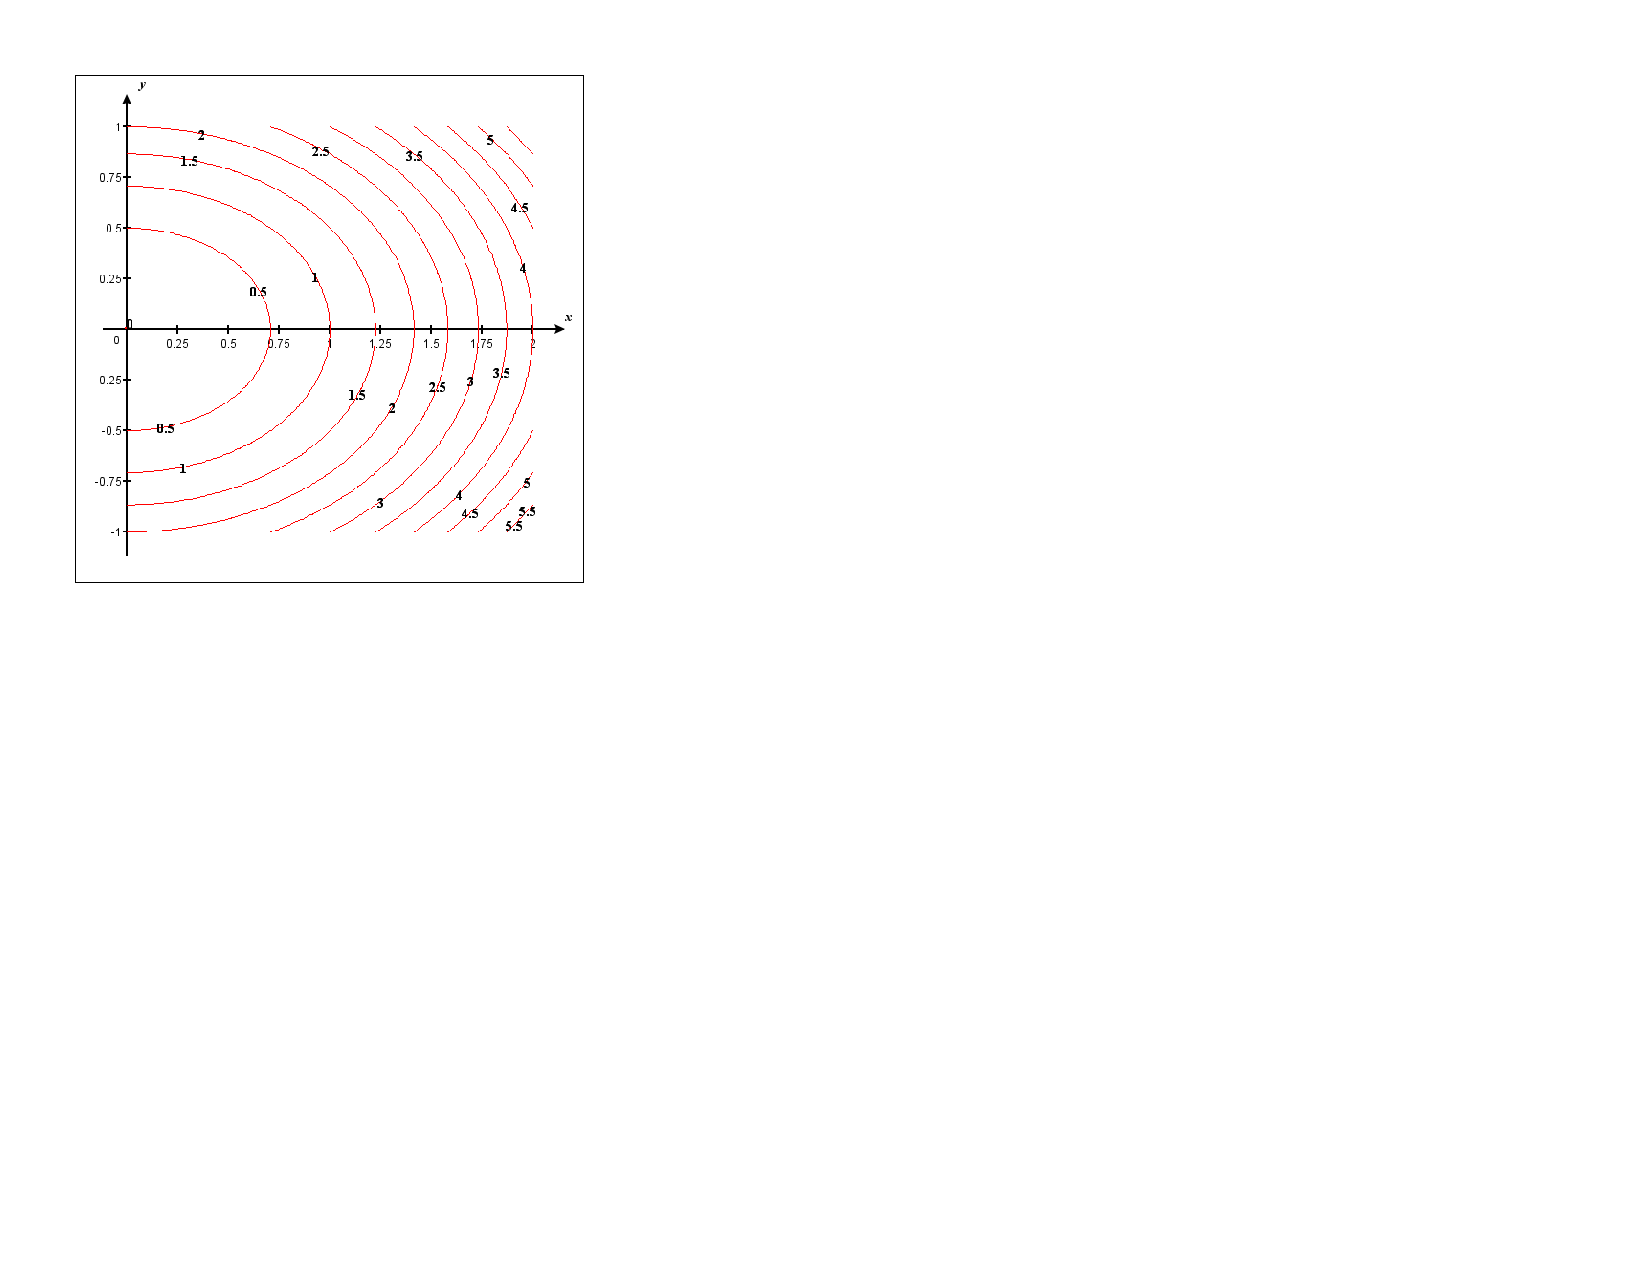
\includegraphics[scale=1]{contour.pdf}
\end{center}

Use this to give an approximation for $\frac{\partial f}{\partial x}(1,0)$.

\includegraphics[scale=0.5]{start.pdf}
{{{1\linewidth}{The slope is approximately 2.  Note: You should use the level curve which passes through $(1,0)$ as well as one which is close to $(1,0)$ to \underline{estimate} the slope.}}}
\includegraphics[scale=0.5]{end.pdf}


\end{enumerate}

\end{document}